\section{Theory}
\label{section: Chapter4/theory}

Test theory for chapter 4

\begin{figure}[h]
    \centering
    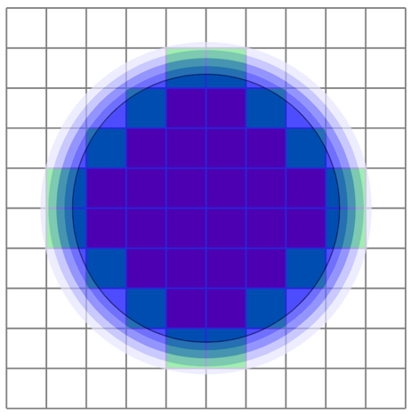
\includegraphics[width=0.5\linewidth]{Chapter4/figures/blue_circle.png}
    \caption{Multi-resolution solution algorithm.}
    \label{fig:lorem1}
\end{figure}

\begin{figure}[h]
    \centering
    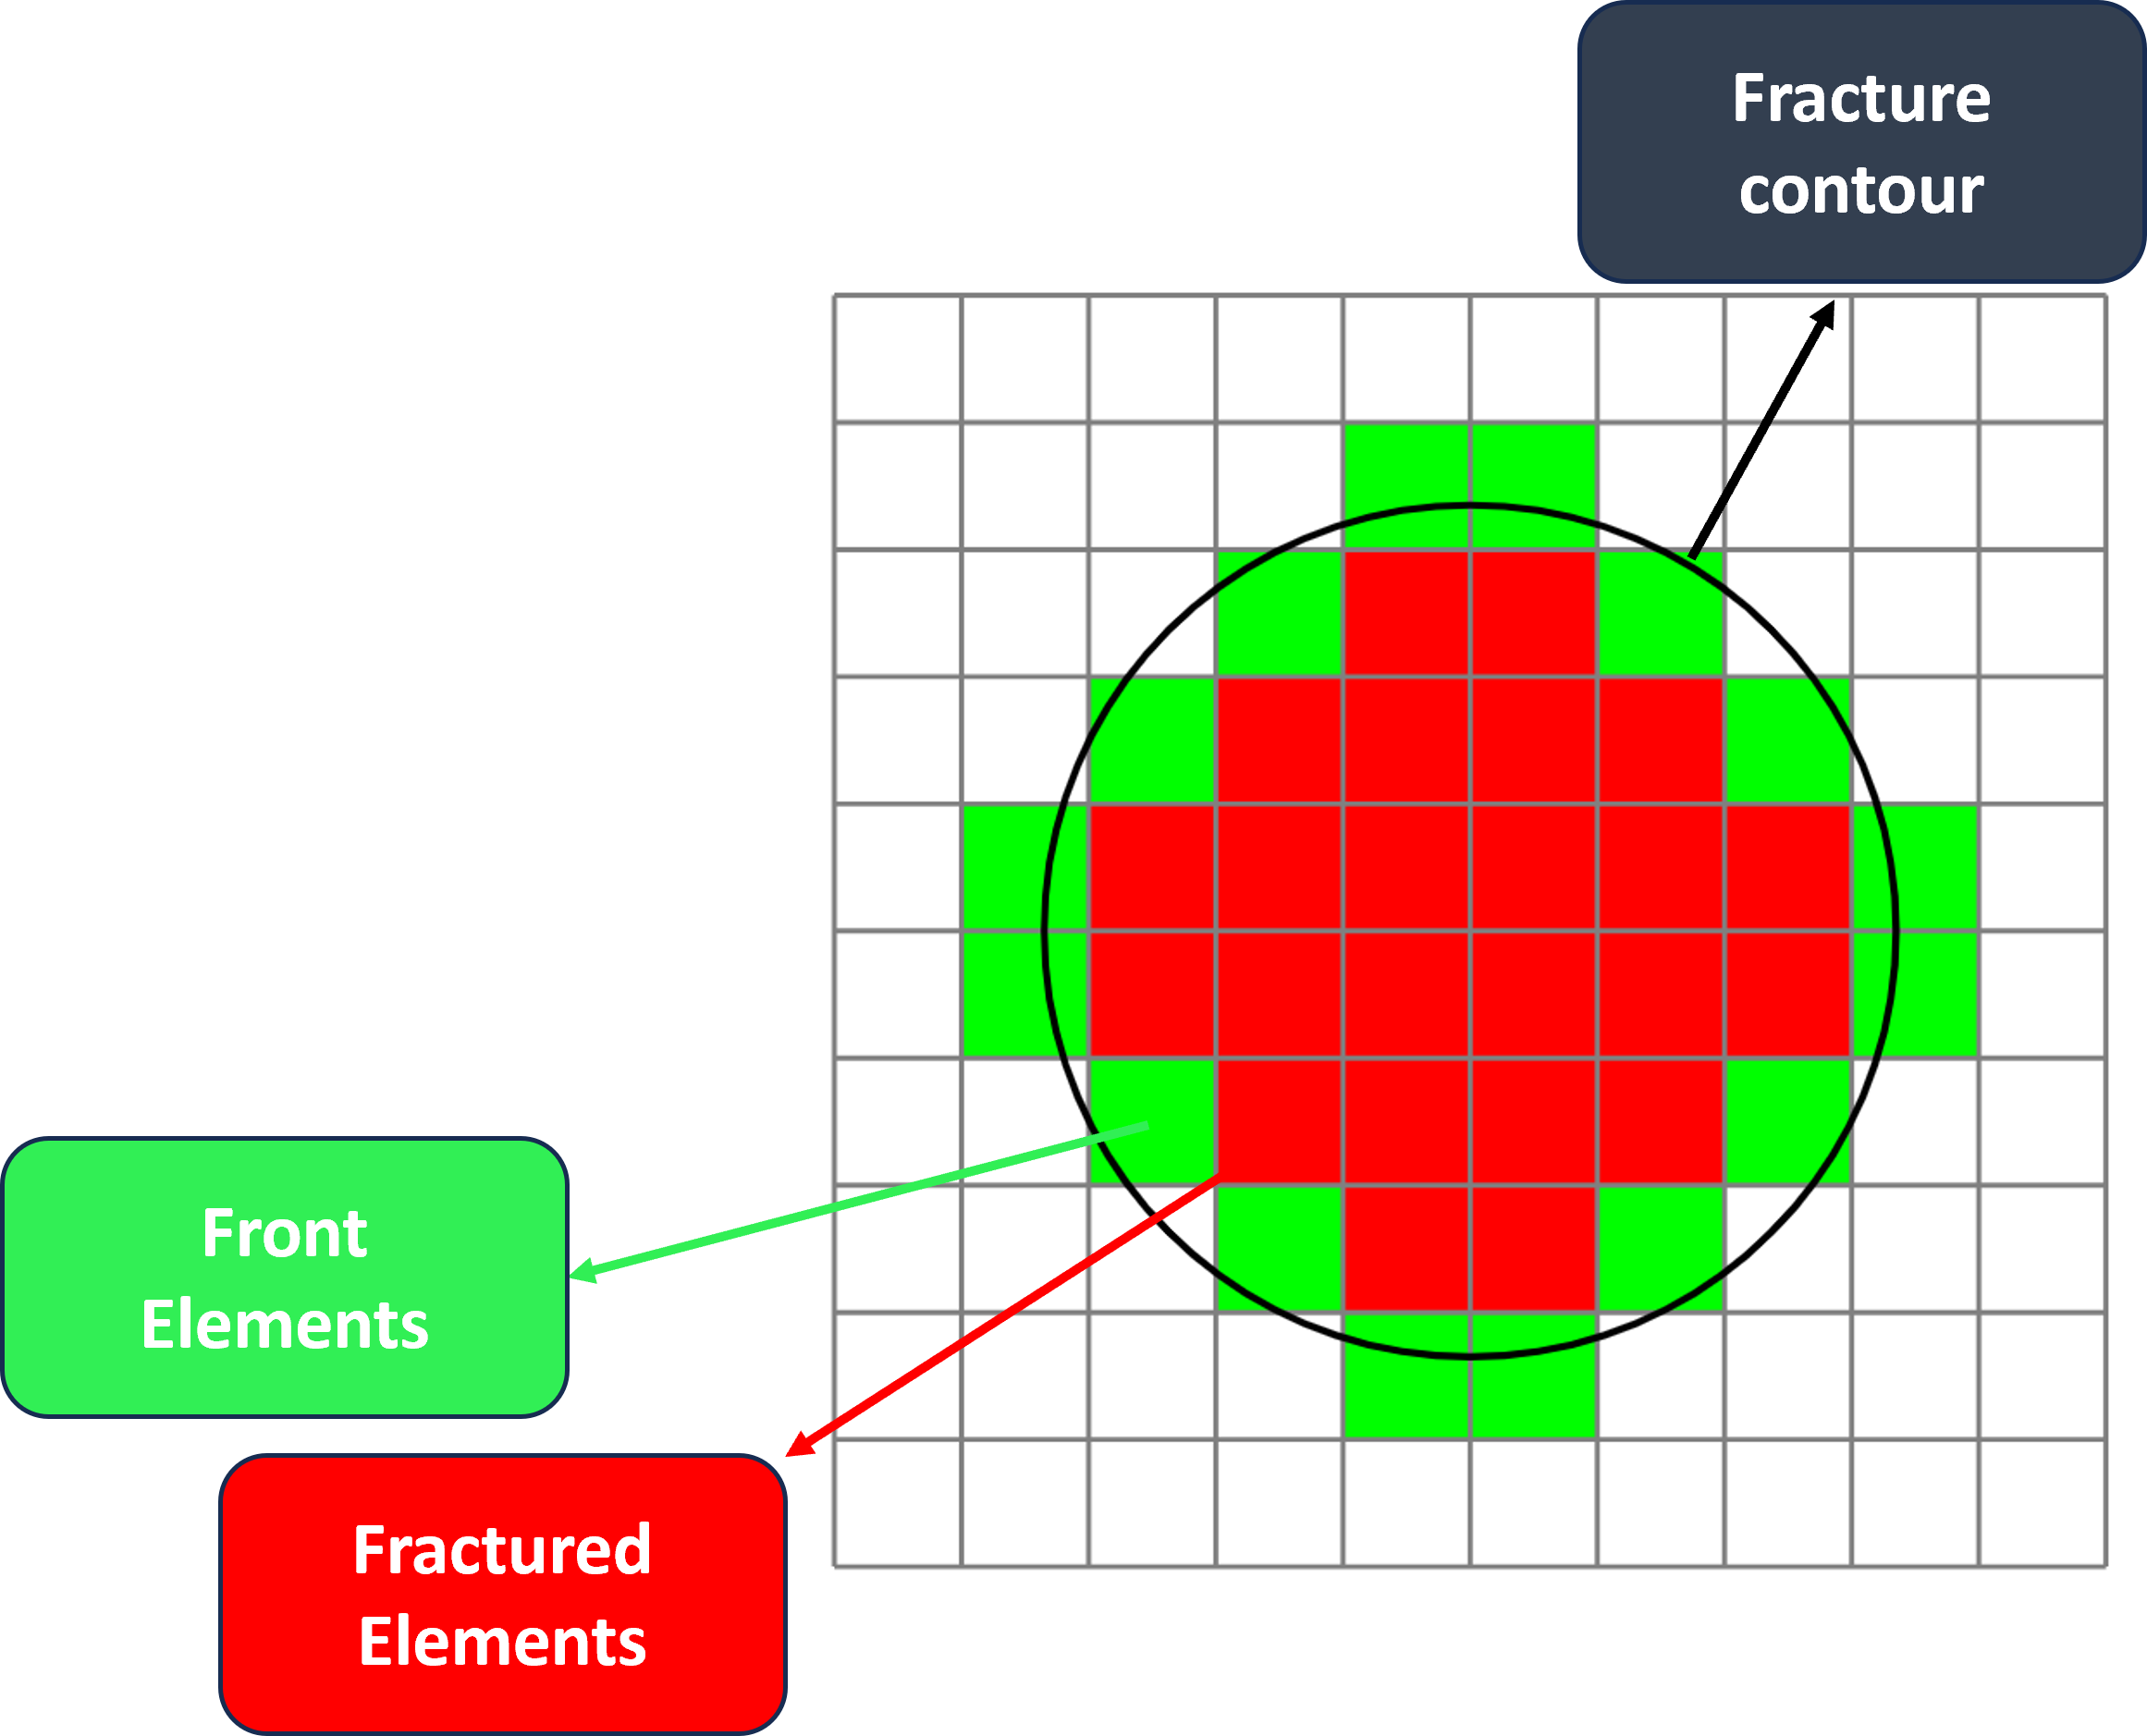
\includegraphics[width=\linewidth]{Chapter4/figures/penny_with_descriptions.png}
    \caption{Multi-resolution solution algorithm.}
    \label{fig:lorem4}
\end{figure}

\begin{figure}[h]
    \centering
    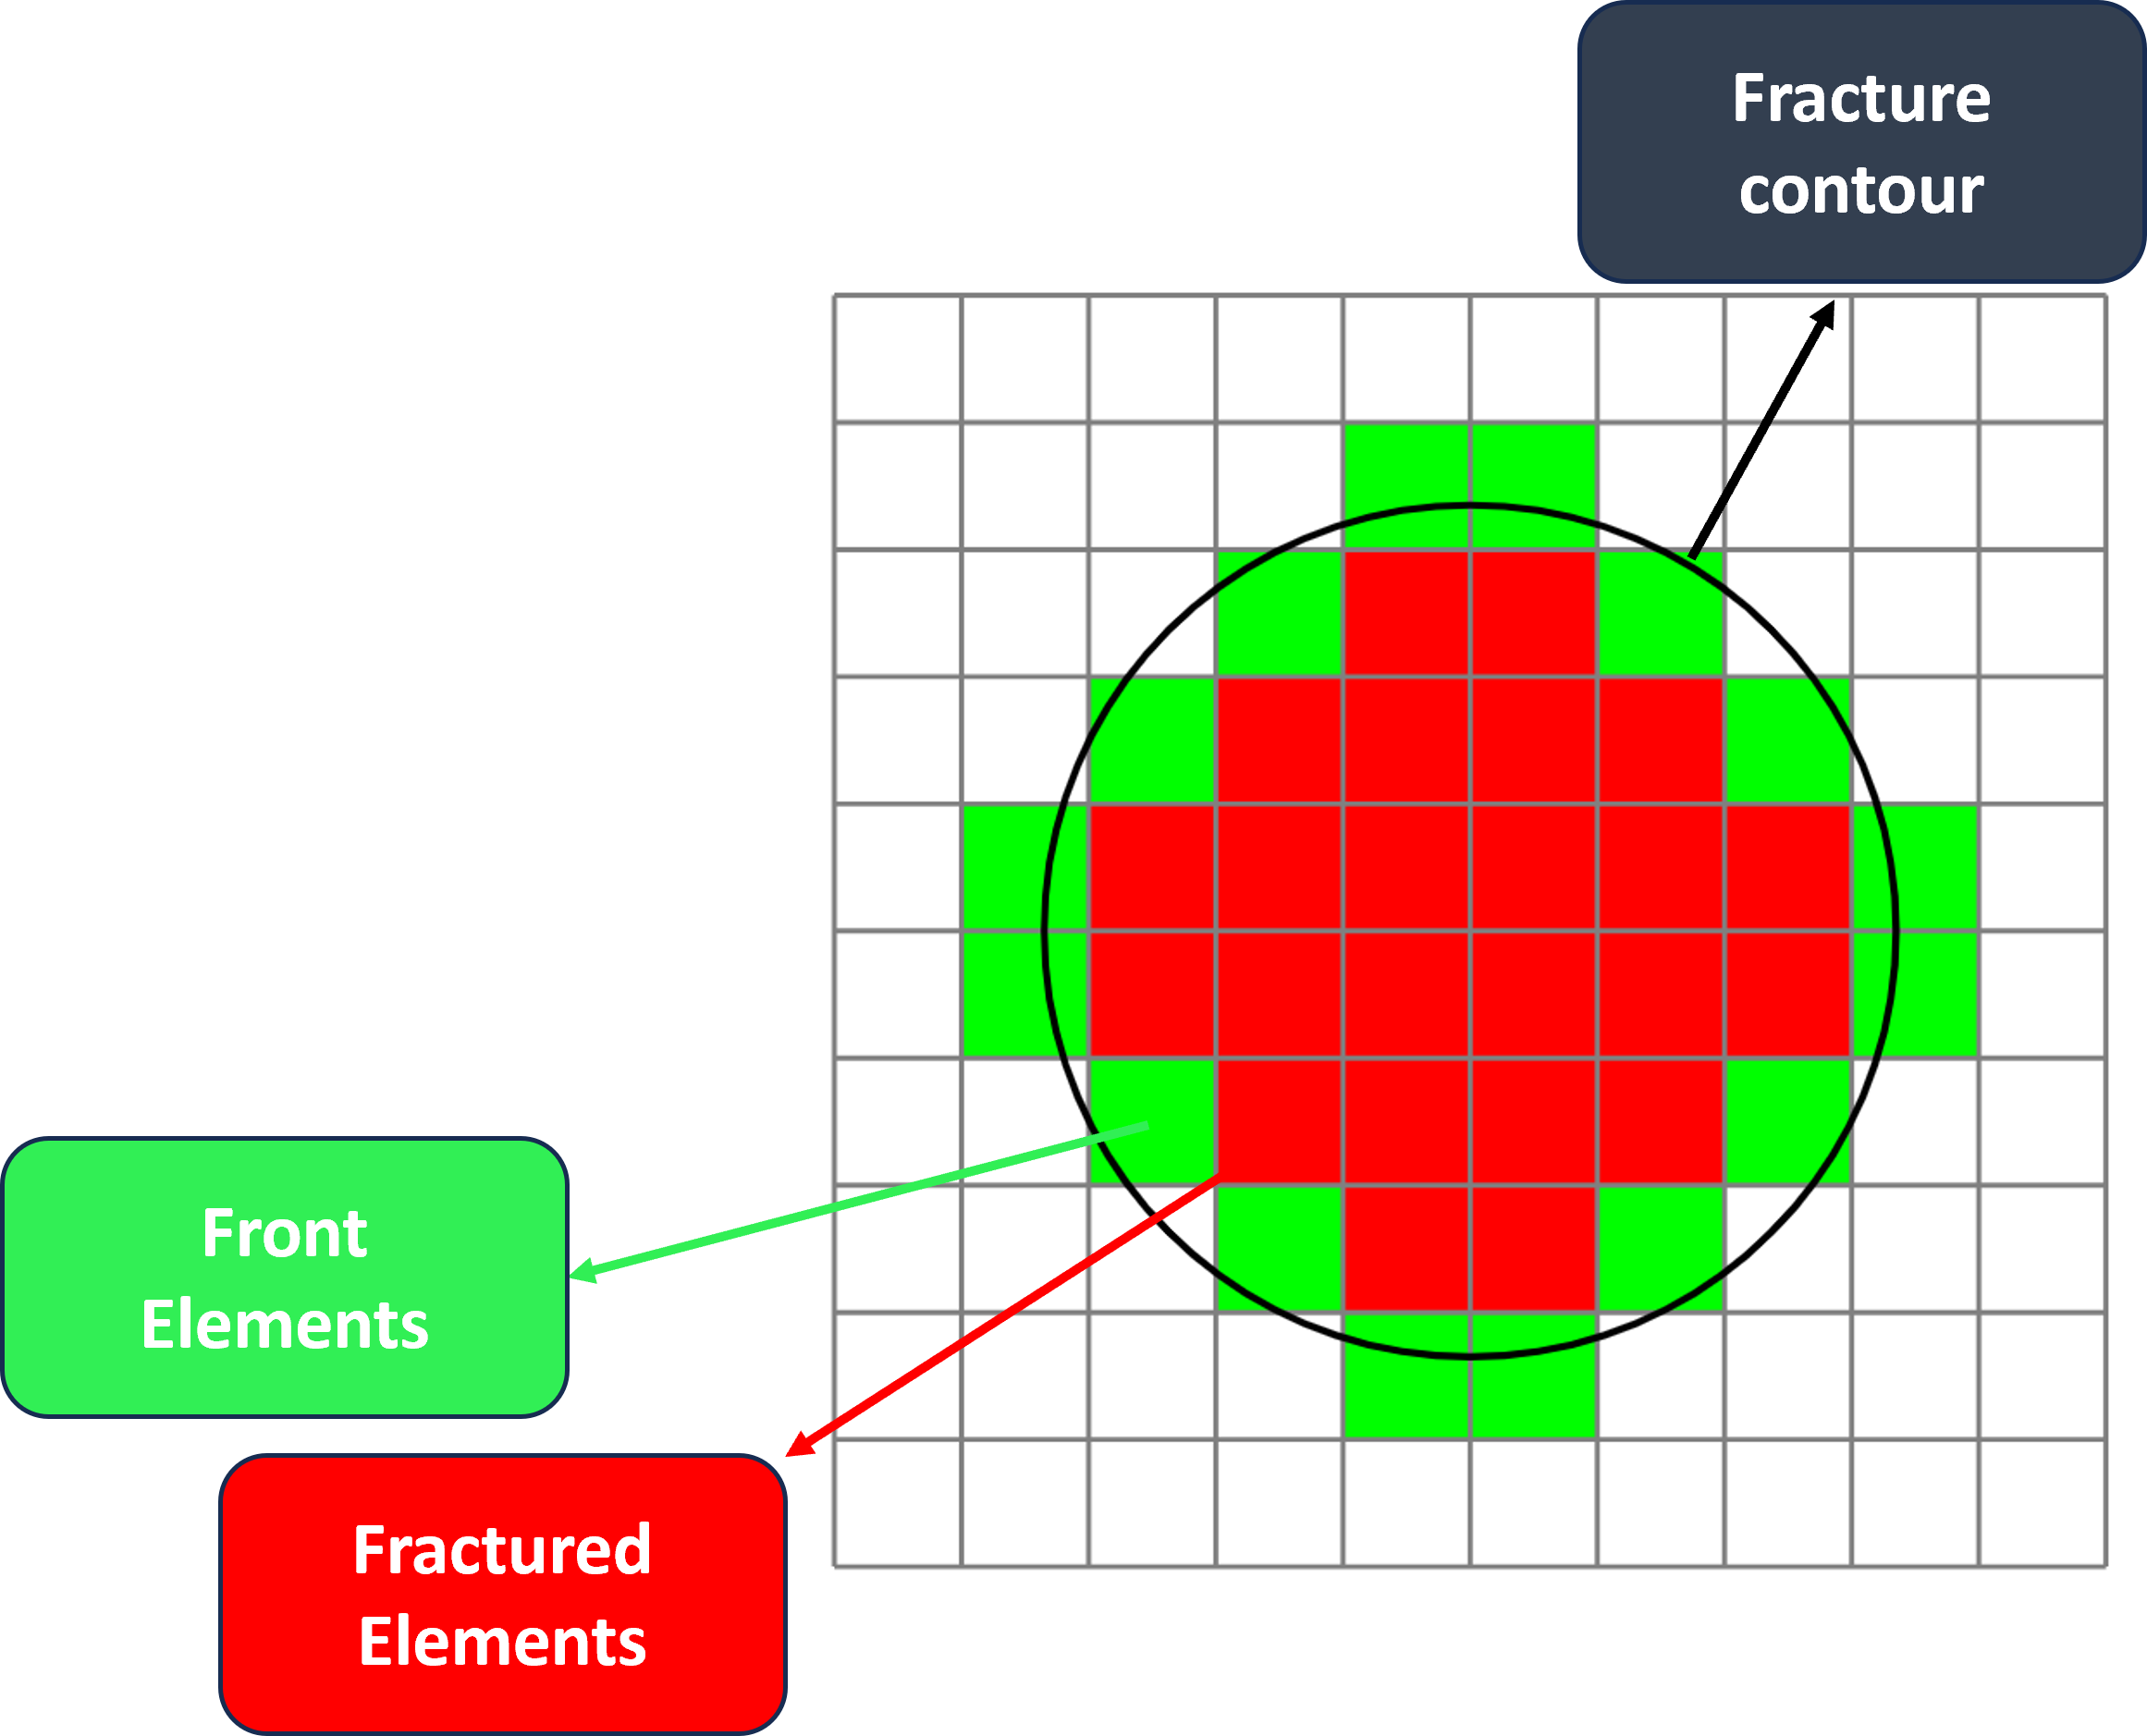
\includegraphics[width=\linewidth]{Chapter4/figures/penny_with_descriptions.png}
    \caption{Multi-resolution solution algorithm.}
    \label{fig:lorem4}
\end{figure}

\begin{figure}[h]
    \centering
    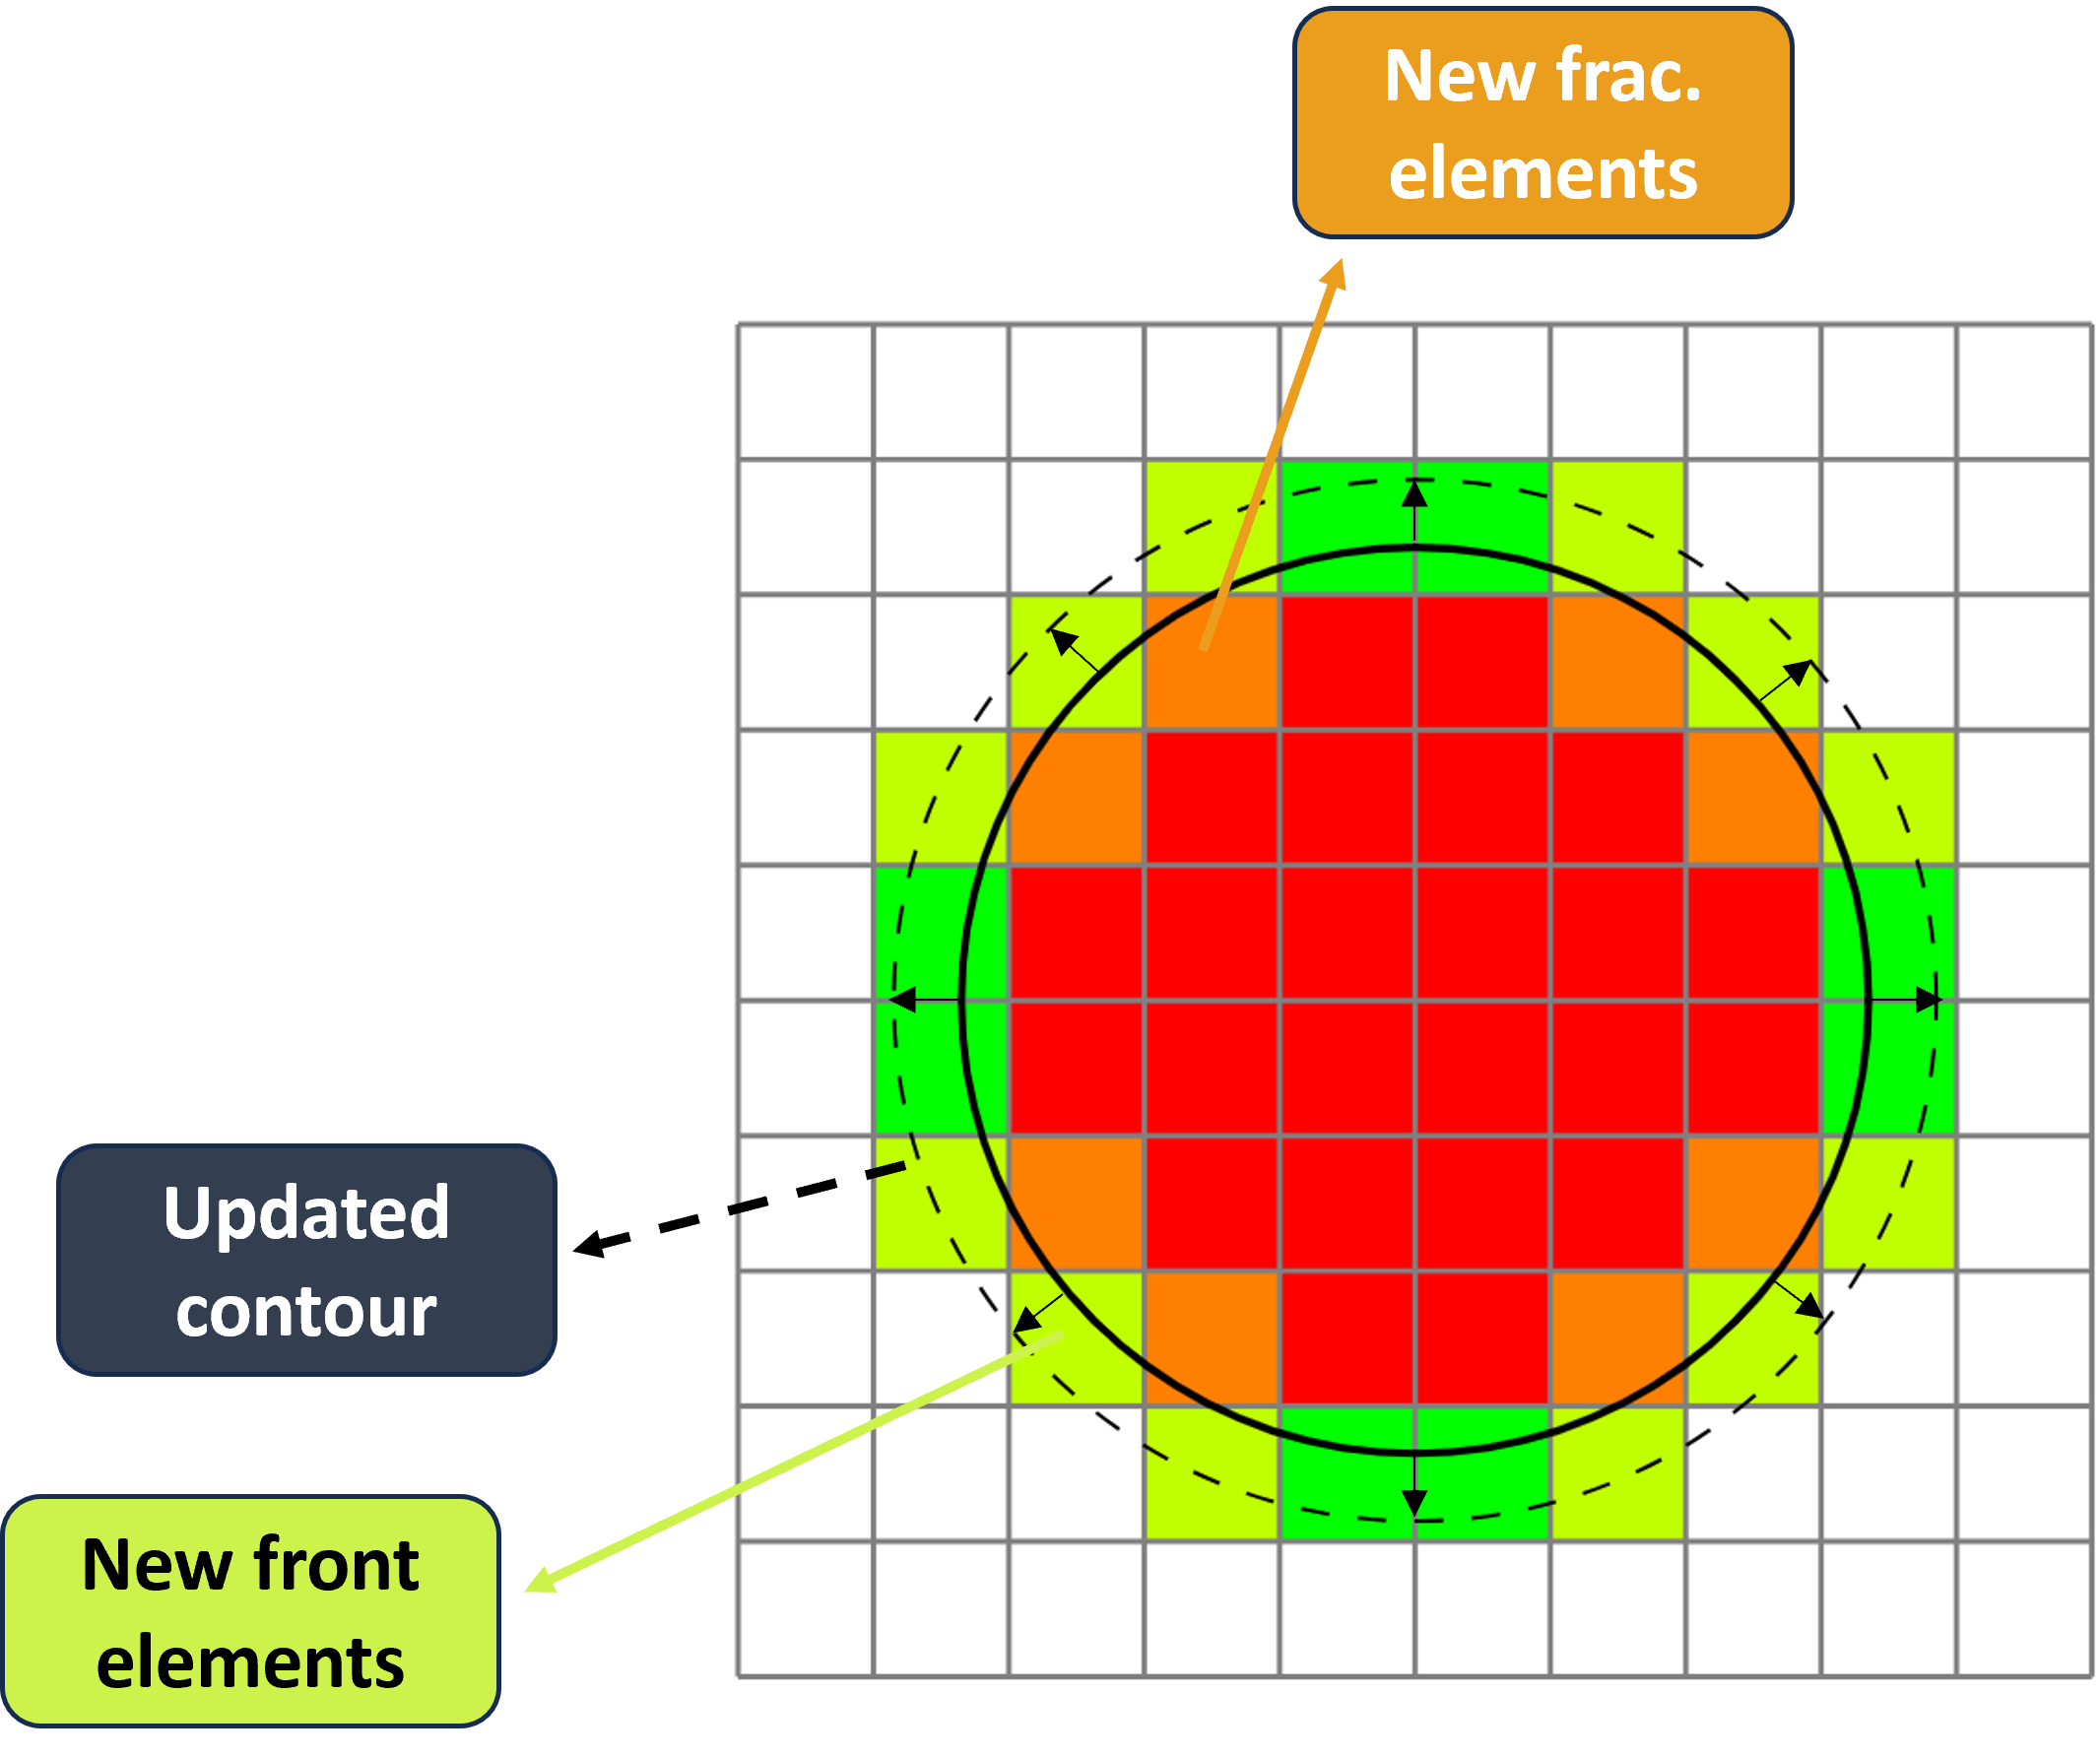
\includegraphics[width=\linewidth]{Chapter4/figures/larger_penny_with_descriptions.png}
    \caption{Multi-resolution solution algorithm.}
    \label{fig:lorem2}
\end{figure}

\begin{figure}[h]
    \centering
    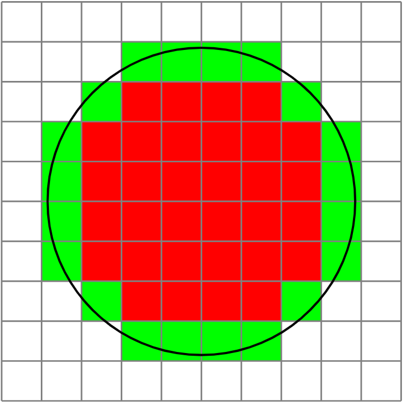
\includegraphics[width=0.5\linewidth]{Chapter4/figures/larger_penny.png}
    \caption{Multi-resolution solution algorithm.}
    \label{fig:lorem3}
\end{figure}

\begin{figure}[h]
    \centering
    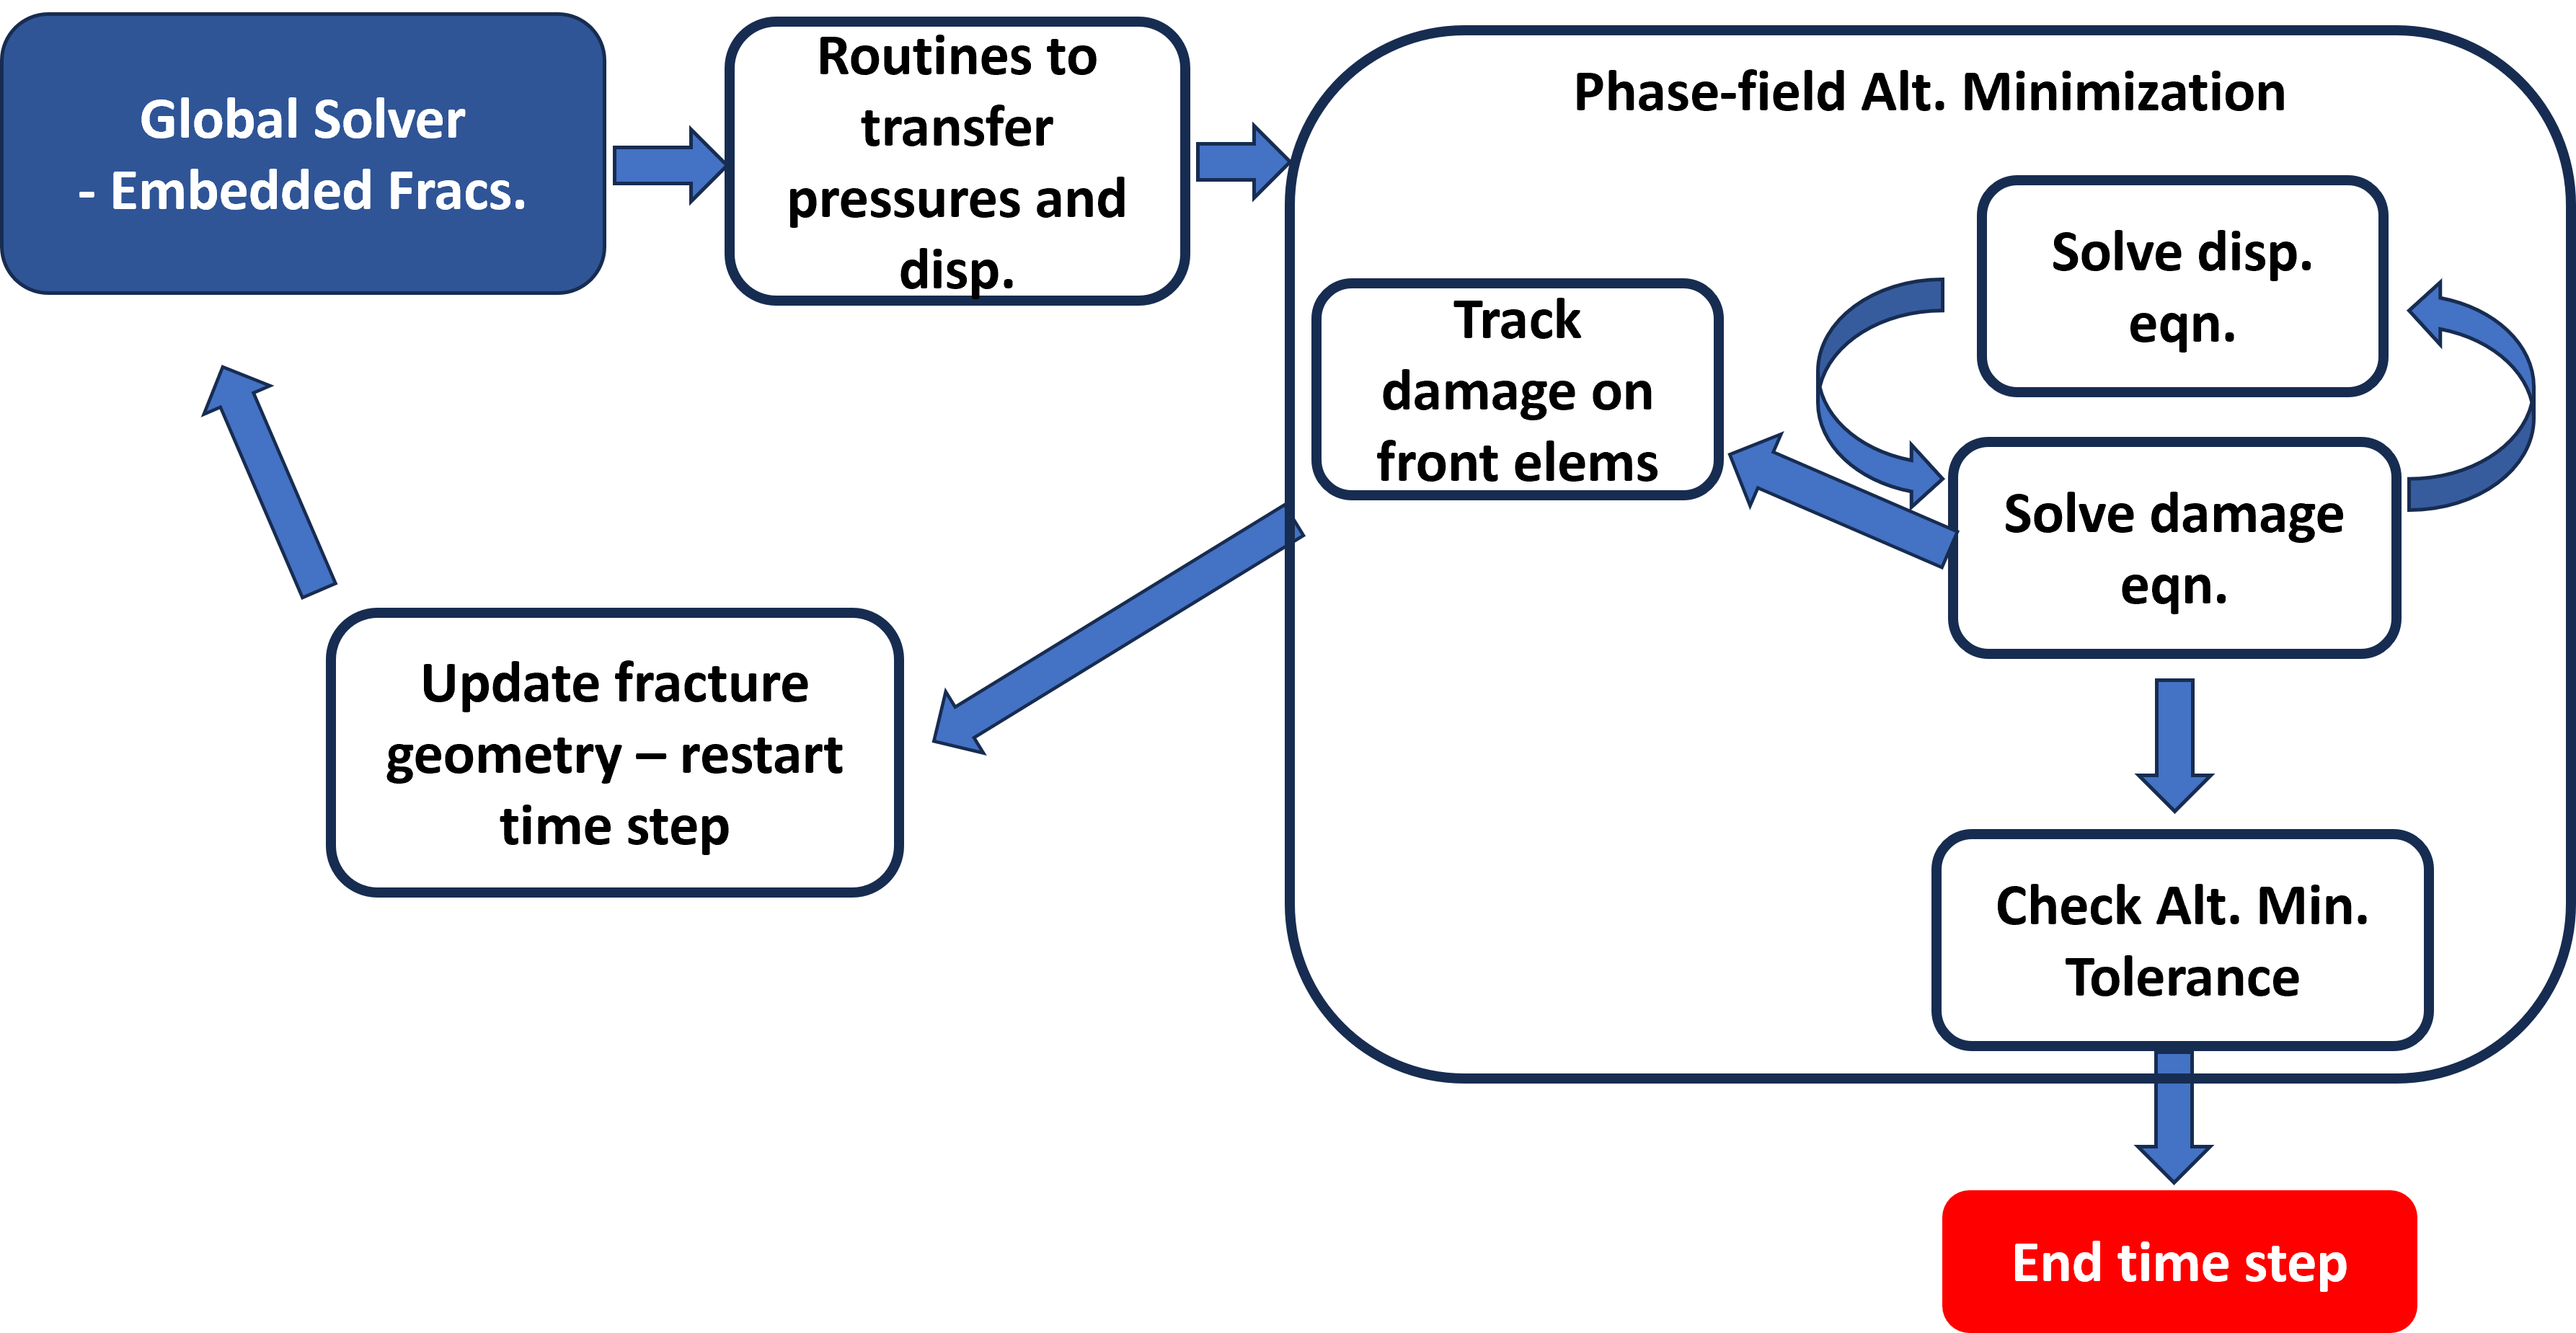
\includegraphics[width=\linewidth]{Chapter4/figures/planar3D_algorithm.png}
    \caption{Multi-resolution solution algorithm.}
    \label{fig:lorem5}
\end{figure}
